\documentclass[notitlepage,11pt]{article}


% Packages
% --------
%	 Necessary
\usepackage{geometry} 						% geometry - page dimensions
\usepackage[parfill]{parskip}				% parskip - to use blank line to sep paragraphs
\usepackage{titling}						% title formatting
\usepackage{enumitem}

\usepackage{amsmath}						% AMS - math, fonts, symbols, theorem
\usepackage{amsfonts}
\usepackage{amssymb}
\usepackage{amsthm}
\usepackage{mathtools}						% mathtools - \coloneqq

\usepackage{listings}						% listings - prints source code

\usepackage{hyperref}						% hyperref - urls and things

\usepackage{tikz}							% tikz - graphs

% 	Additional
\usepackage{graphicx}						% graphicx - importing graphics from file
\usepackage{subcaption}
\captionsetup[subfigure]{labelformat=empty}
\usepackage[T1]{fontenc}
\usepackage[utf8]{inputenc}
\usepackage{helvet}
\renewcommand{\familydefault}{\sfdefault}	% change to helvetica

\usepackage{forest}							% forest - easy trees
\usepackage{tikzsymbols}					% tikzsymbols - just adds some symbols
% tikzlibrary summary: 
% tex.stackexchange.com/questions/42611/list-of-available-tikz-libraries-with-a-short-introduction/491626
\usetikzlibrary{arrows.meta}				% arrows.meta - customizable arrow tips
\usetikzlibrary{er}							% entity-relationship diagrams
\usetikzlibrary{positioning} 				% relative positioning
\usetikzlibrary{shadows}
\usetikzlibrary{shapes}

\usepackage{xcolor}							% xcolor - adds additional colors

\usepackage{marginnote}						% marginnote - see name

\usepackage{multirow}						% multirow - sort of a tabular environment of text
\usepackage{bigdelim}						% bigdelim - used with multirow once to make brackets on tables
\usepackage{array}							% array - extends arrary and tabular environment
\usepackage{makecell}						% makecell - adjust cell cizes within tabular environment

\usepackage[bottom]{footmisc}				% comment out to make footnotes not appear at bottom of page

% Customizations

\pretitle{\begin{center}\Large\bfseries}		% titling format
\posttitle{\par\end{center}\vskip 0cm}
\preauthor{\begin{center}\large}
\postauthor{\end{center}}
\predate{\par\normalsize\centering}
\postdate{\par}

\newtheoremstyle{customnumber} % name
	{}% space above
	{}% space below
	{\normalfont}% body font
	{}% indent 
	{\bfseries}% head font
	{:}% punctuation between head/body
	{ }% space after head: " " = normal whitespace
	{\thmname{#1}\thmnote{ #3}}% head format

\newtheoremstyle{named}
	{}
	{}
	{\normalfont}
	{}
	{\bfseries}
	{.}
	{ }
	{\thmnote{#3}}

\theoremstyle{customnumber}
\newtheorem*{exercise}{Exercise}

\theoremstyle{definition}
\newtheorem{defi}{Definition}

\newtheorem{ex}{Example}[section]

\theoremstyle{named}
\newtheorem*{namedtheorem}{}

\newenvironment{absolutelynopagebreak}
	{\par\nobreak\vfil\penalty0\vfilneg\vtop\bgroup}
	{\par\xdef\tpd{\the\prevdepth}\egroup\prevdepth=\tpd}
	
\newcommand{\indep}{\raisebox{0.05em}{\rotatebox[origin=c]{90}{$\models$}}}

\newcommand{\stcomp}[1]{{#1}^\complement}


\lstset{tabsize=3, numbers=left, basicstyle=\ttfamily, escapeinside=~~, xleftmargin=-1cm}
\let\origthelstnumber\thelstnumber
\makeatletter
\newcommand*\Suppressnumber{%
	\lst@AddToHook{OnNewLine}{%
		\let\thelstnumber\relax%
		\advance\c@lstnumber-\@ne\relax%
	}%
}
\newcommand*\Reactivatenumber{%
	\lst@AddToHook{OnNewLine}{%
		\let\thelstnumber\origthelstnumber%
		\advance\c@lstnumber\@ne\relax%
	}%
}
\makeatother

\graphicspath{{./UI/}}

\geometry{margin=1in}

\setitemize{noitemsep,topsep=-2pt,parsep=-2pt,partopsep=-2pt}

\title{COMP 3700 Project 1}
\author{Tripp Isbell\\
	\texttt{cai0004@auburn.edu}\\
	\href{https://github.com/Carbonationalism/COMP3700/tree/master/activities/Project1}{Github}}
\date{}
\setlength{\droptitle}{-2cm}
\pagenumbering{gobble}

\begin{document}
\maketitle

\section{User Story: Add Product}
\textbf{Use Case:} add a product into the system\\
	\textbf{Actors:} employees\\
	\textbf{Goals:} update database to include new product\\
	\textbf{Related use cases:} adding a customer to the database or recording a transaction (below)
	\textbf{Preconditions:} interface is functional and connected to underlying database\\
	\textbf{Postconditions:} The product database is updated with the item\\
	\textbf{Steps:}
		\begin{itemize}
		\item[(1)] the user clicks a button to display the product database
		\item[(2)] the system displays the database
		\item the user clicks add product
		\item[(3)] the system displays a screen with text fields for the product info
		\item the user enters the information and clicks an add button
		\item[(4)] the system updates the database and displays a confirmation message
		\item the user clicks confirm 
		\item[(1)] the system returns to the main menu
		\end{itemize}
\begin{figure}[h]
	\begin{subfigure}{.5\textwidth}
	\centering
	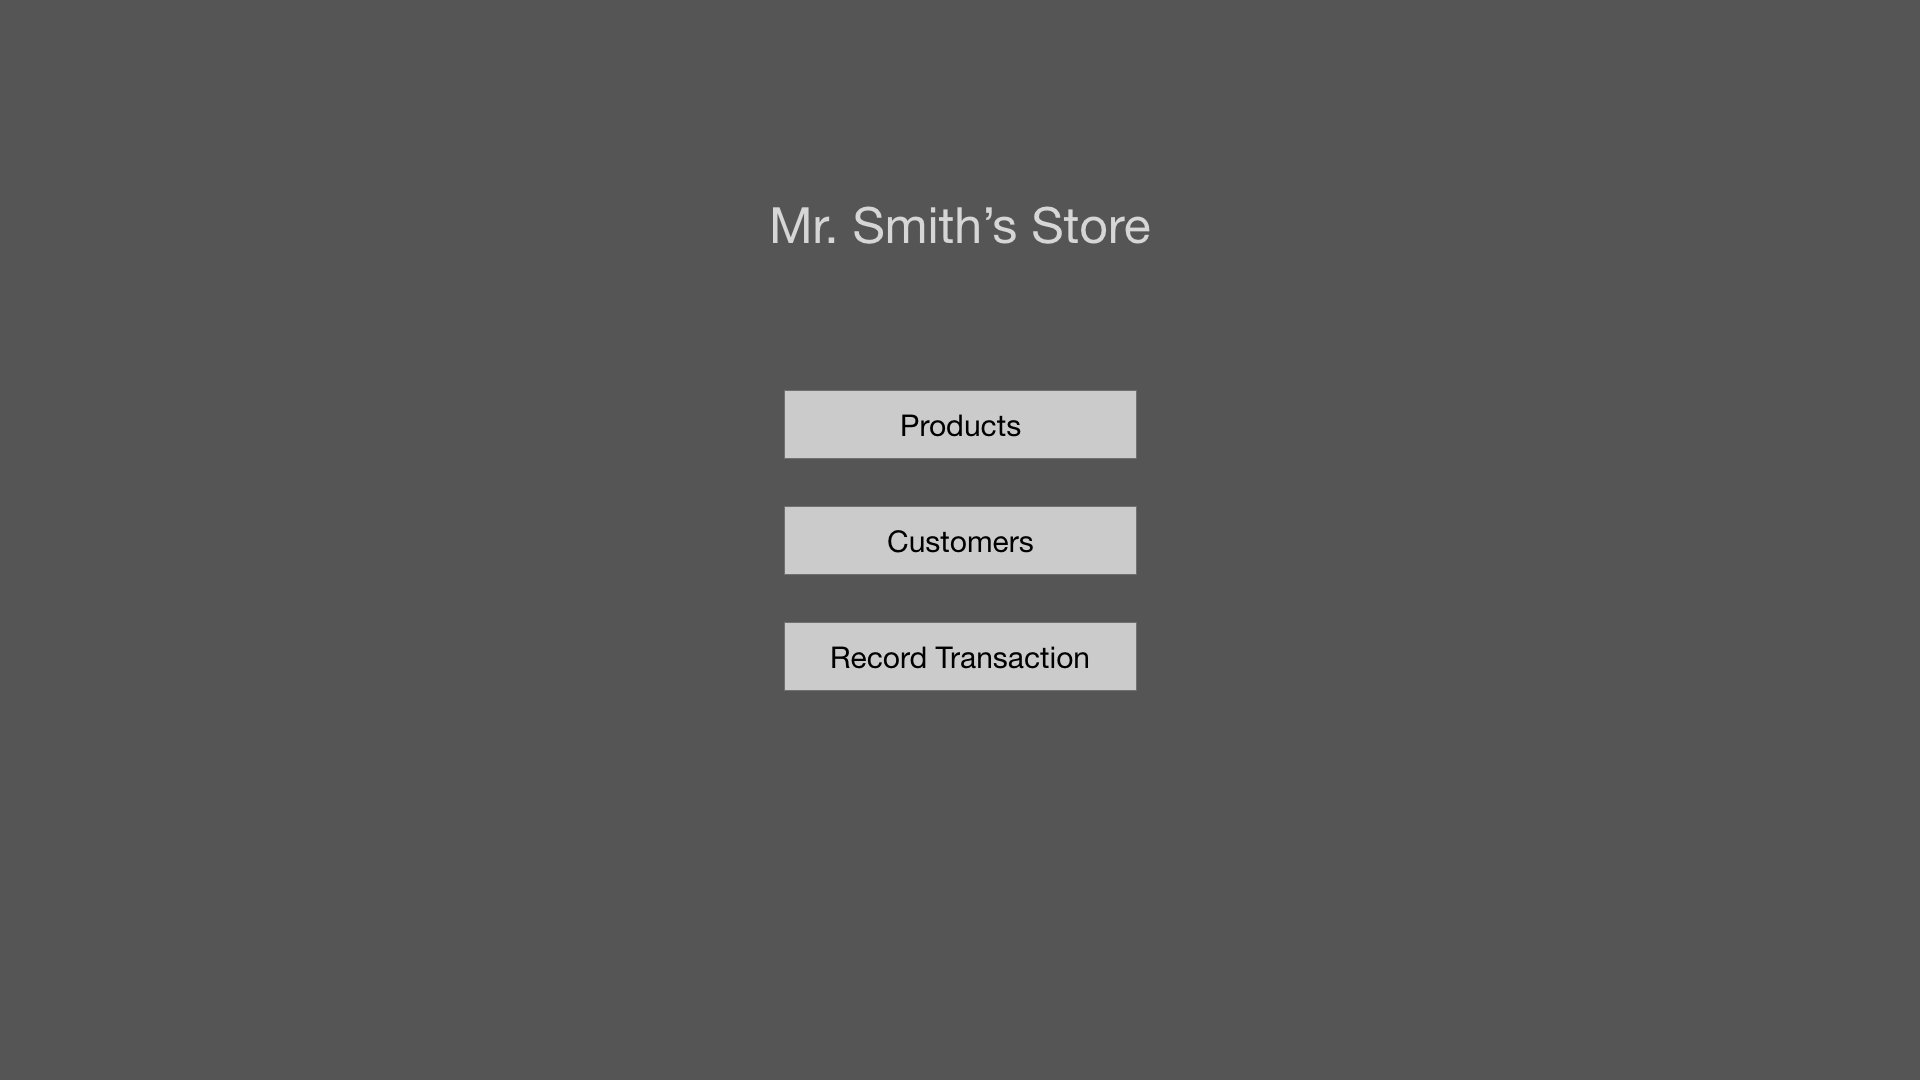
\includegraphics[scale=0.12]{MainMenu}
	\caption{(1)}
	\end{subfigure}%
	\begin{subfigure}{.5\textwidth}
	\centering
	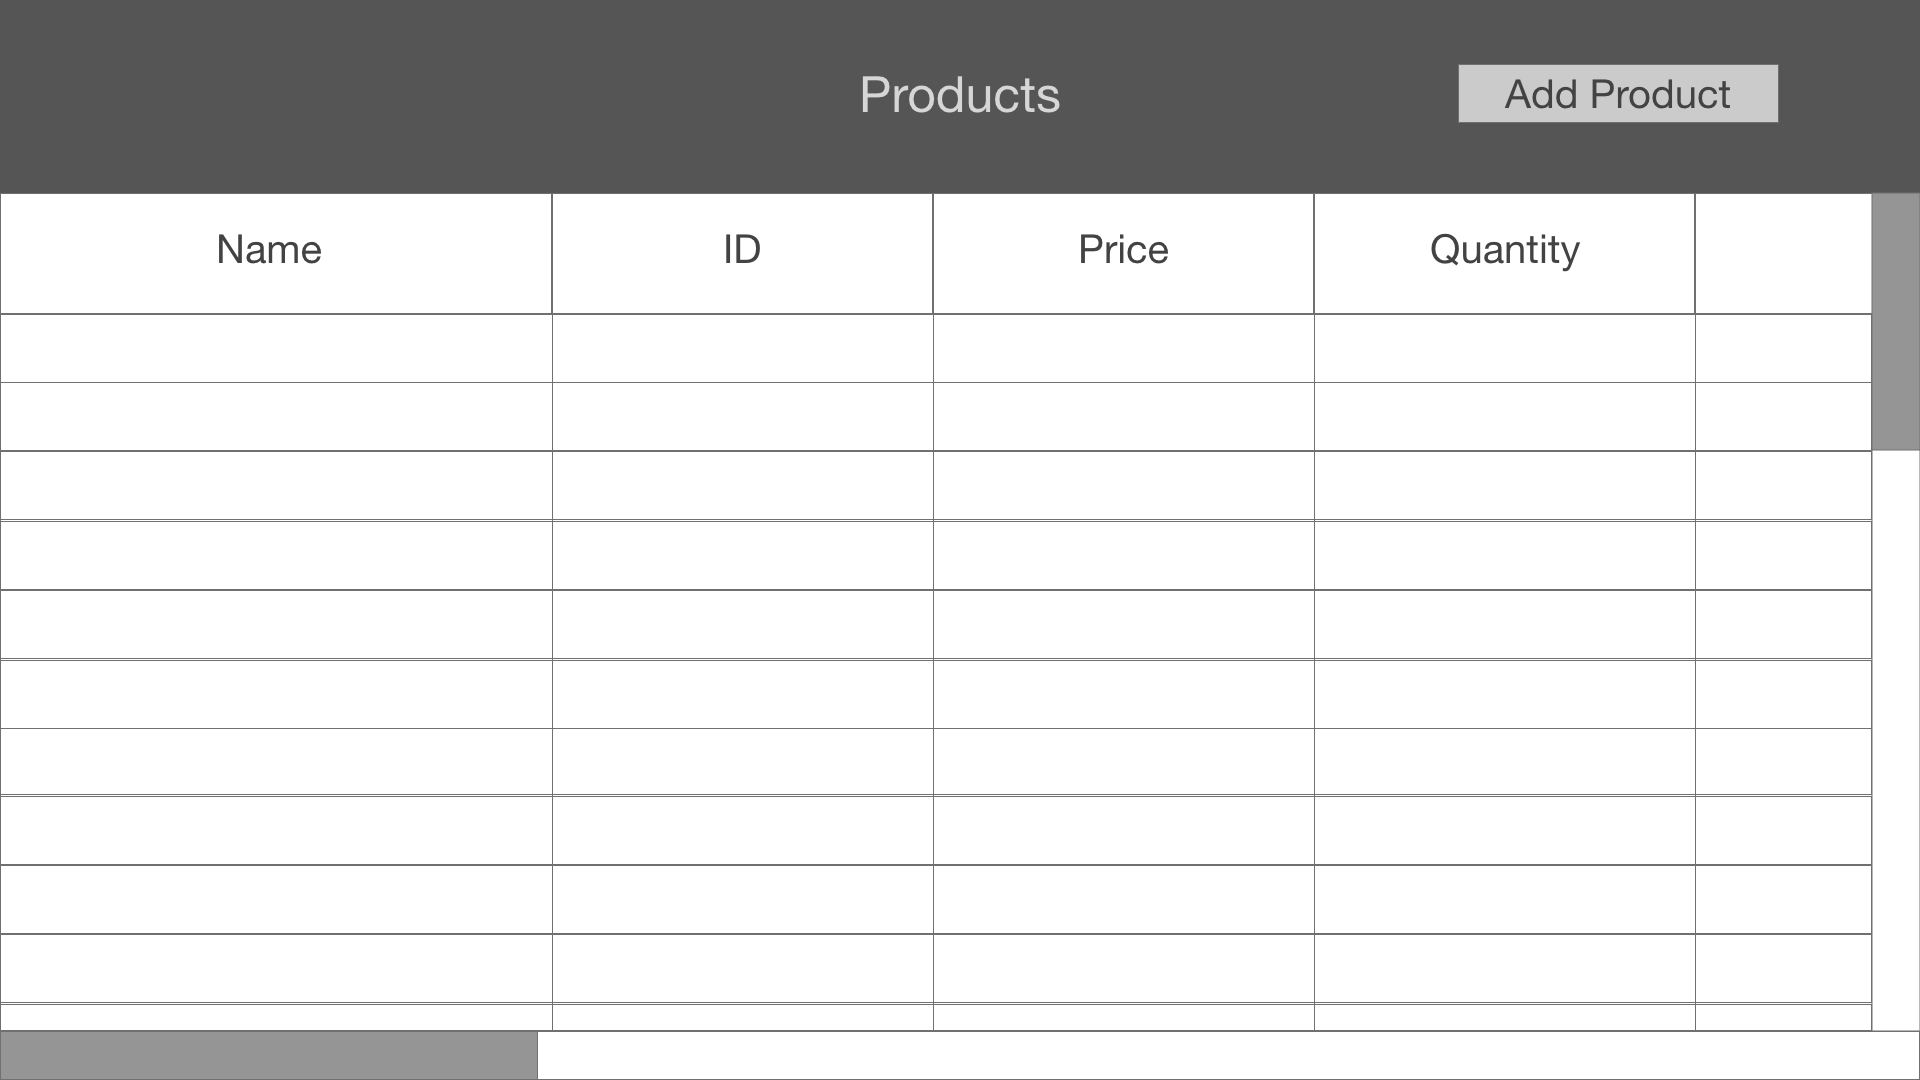
\includegraphics[scale=0.12]{AddProduct}
	\caption{(2)}
	\end{subfigure}
\end{figure}
\begin{figure}[h]
	\begin{subfigure}{.5\textwidth}
	\centering
	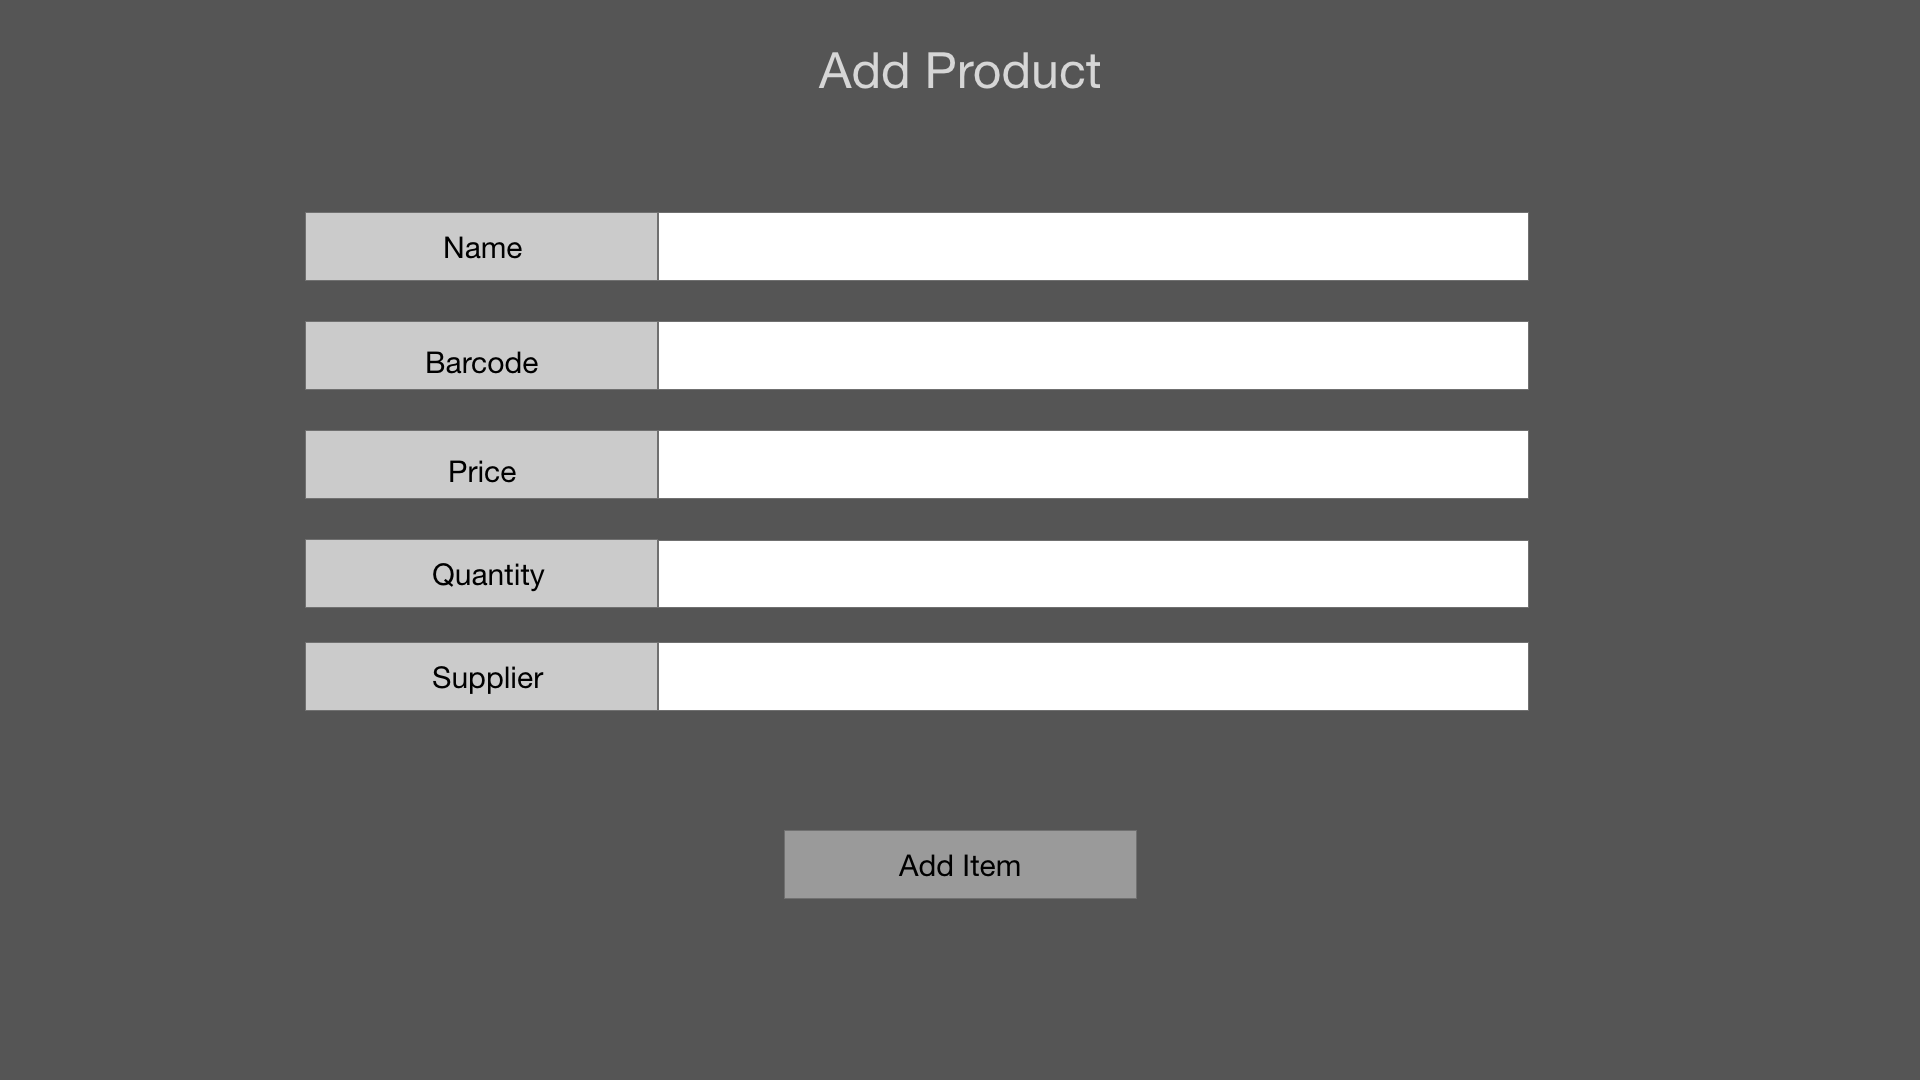
\includegraphics[scale=0.12]{ProdInfo}
	\caption{(3)}
	\end{subfigure}%
	\begin{subfigure}{.5\textwidth}
	\centering
	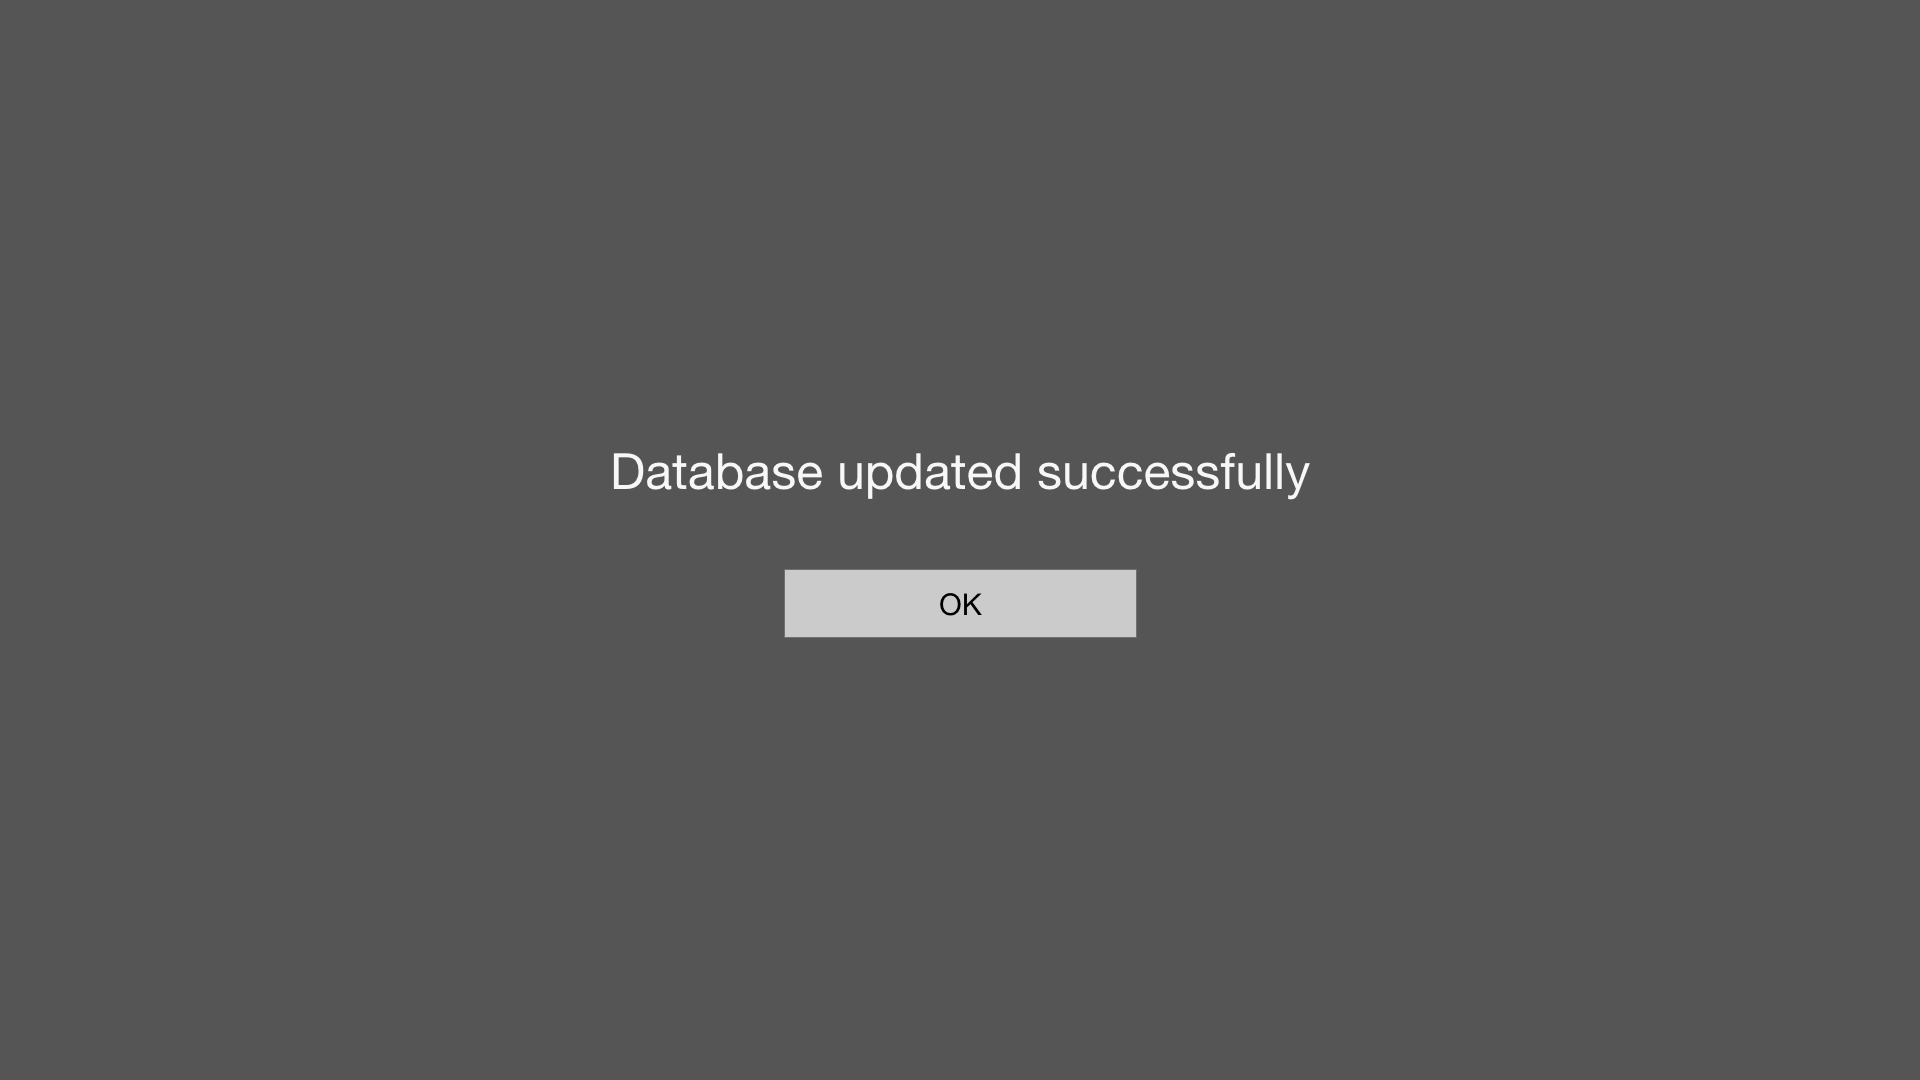
\includegraphics[scale=0.12]{Success}
	\caption{(4)}
	\end{subfigure}
\end{figure}

\textbf{Use Case:} update a product in the system\\
\textbf{Actors:} employees\\
\textbf{Goals:} update a product in the database\\
\textbf{Preconditions:} the target product exists in the database\\
\textbf{Postconditions:} the database is updated with desired changes\\
\textbf{steps:}
	\begin{itemize}
		\item[(1)] the user clicks a button to display the product database
		\item[(2)] the system displays the database
		\item the user (double) clicks on the desired field to edit
		\item the system responds by making the field editable
		\item the user enters desired changes and presses enter
		\item the system updates the underlying database as well as the GUI
	\end{itemize}
the (1) and (2) views here are the same (1) and (2) views on the previous page

\textbf{SQL code} to create table, insert, update, and delete
\Suppressnumber
\begin{lstlisting}
CREATE TABLE IF NOT EXISTS Product (
	Barcode integer PRIMARY KEY,
	Name text,
	Price real,
	Quantity real,
	Supplier text);
INSERT INTO Product (Barcode, Name, Price, Quantity, Supplier)
	VALUES (1, 'iphone', 899.99, 50, 'Apple');
UPDATE Product SET 
	Barcode = 1,
	Name = 'iphone',
	Price = 799.99,
	Quantity = 40,
	Supplier = 'Apple' 
WHERE Barcode = 1;
DELETE FROM Product WHERE Barcode = 1;
\end{lstlisting}
\newpage
\section{User Story: Add Customer}
	\textbf{Use case:} add a customer into the system\\
	\textbf{Actors:} employees\\
	\textbf{Goals:} update database to include new customer\\
	\textbf{Related use cases:} adding a product or transaction\\
	\textbf{Preconditions, postconditions:} Same as above just replace "product" with "customer"\\
		\textbf{Steps:}
		\begin{itemize}
		\item[(1)] the user clicks a button to display the customer database
		\item[(2)] the system displays the database
		\item the user clicks a plus button 
		\item[(3)] the system displays a screen with text fields for the customer info
		\item the user enters the information and clicks an add button
		\item[(4)] the system updates the database and displays a confirmation message
		\item the user clicks confirm 
		\item[(1)] the system returns to the main menu
		\end{itemize}
\begin{figure}[h]
	\begin{subfigure}{.5\textwidth}
	\centering
	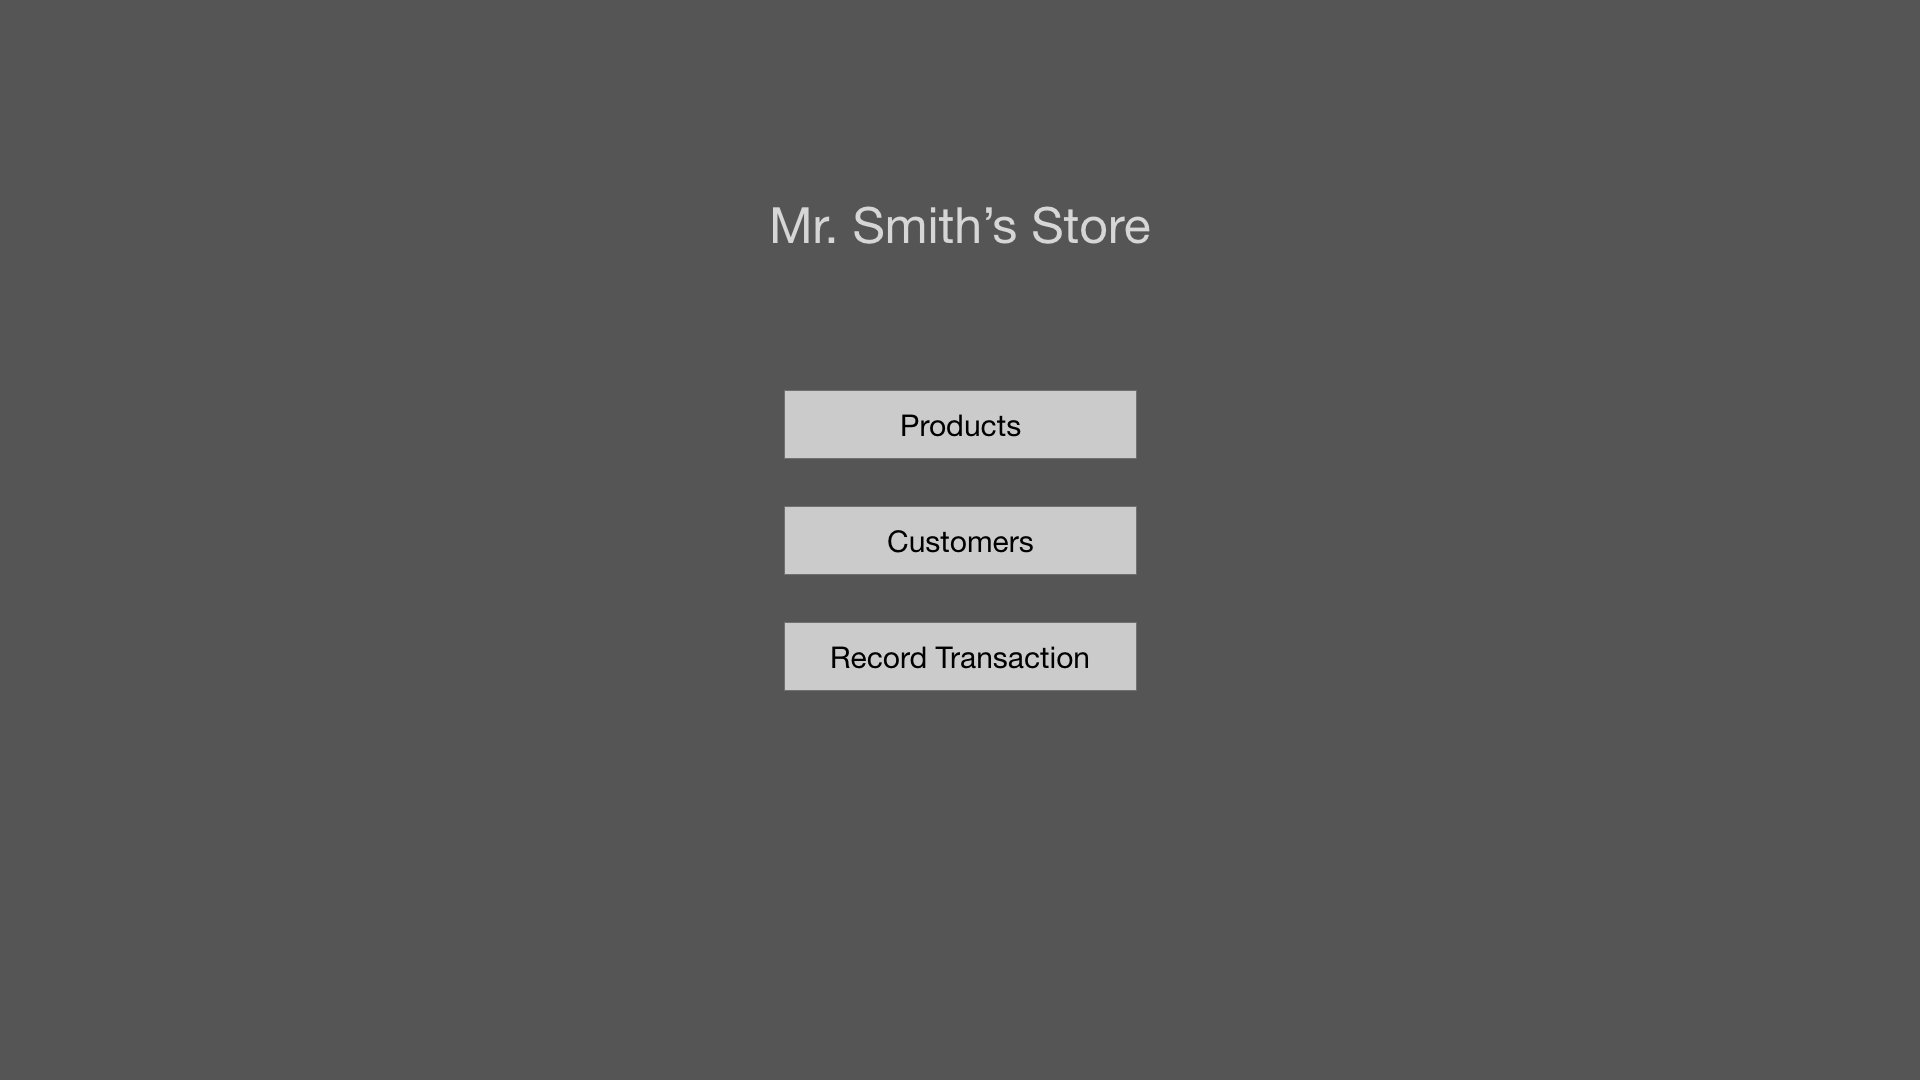
\includegraphics[scale=0.12]{MainMenu}
	\caption{(1)}
	\end{subfigure}%
	\begin{subfigure}{.5\textwidth}
	\centering
	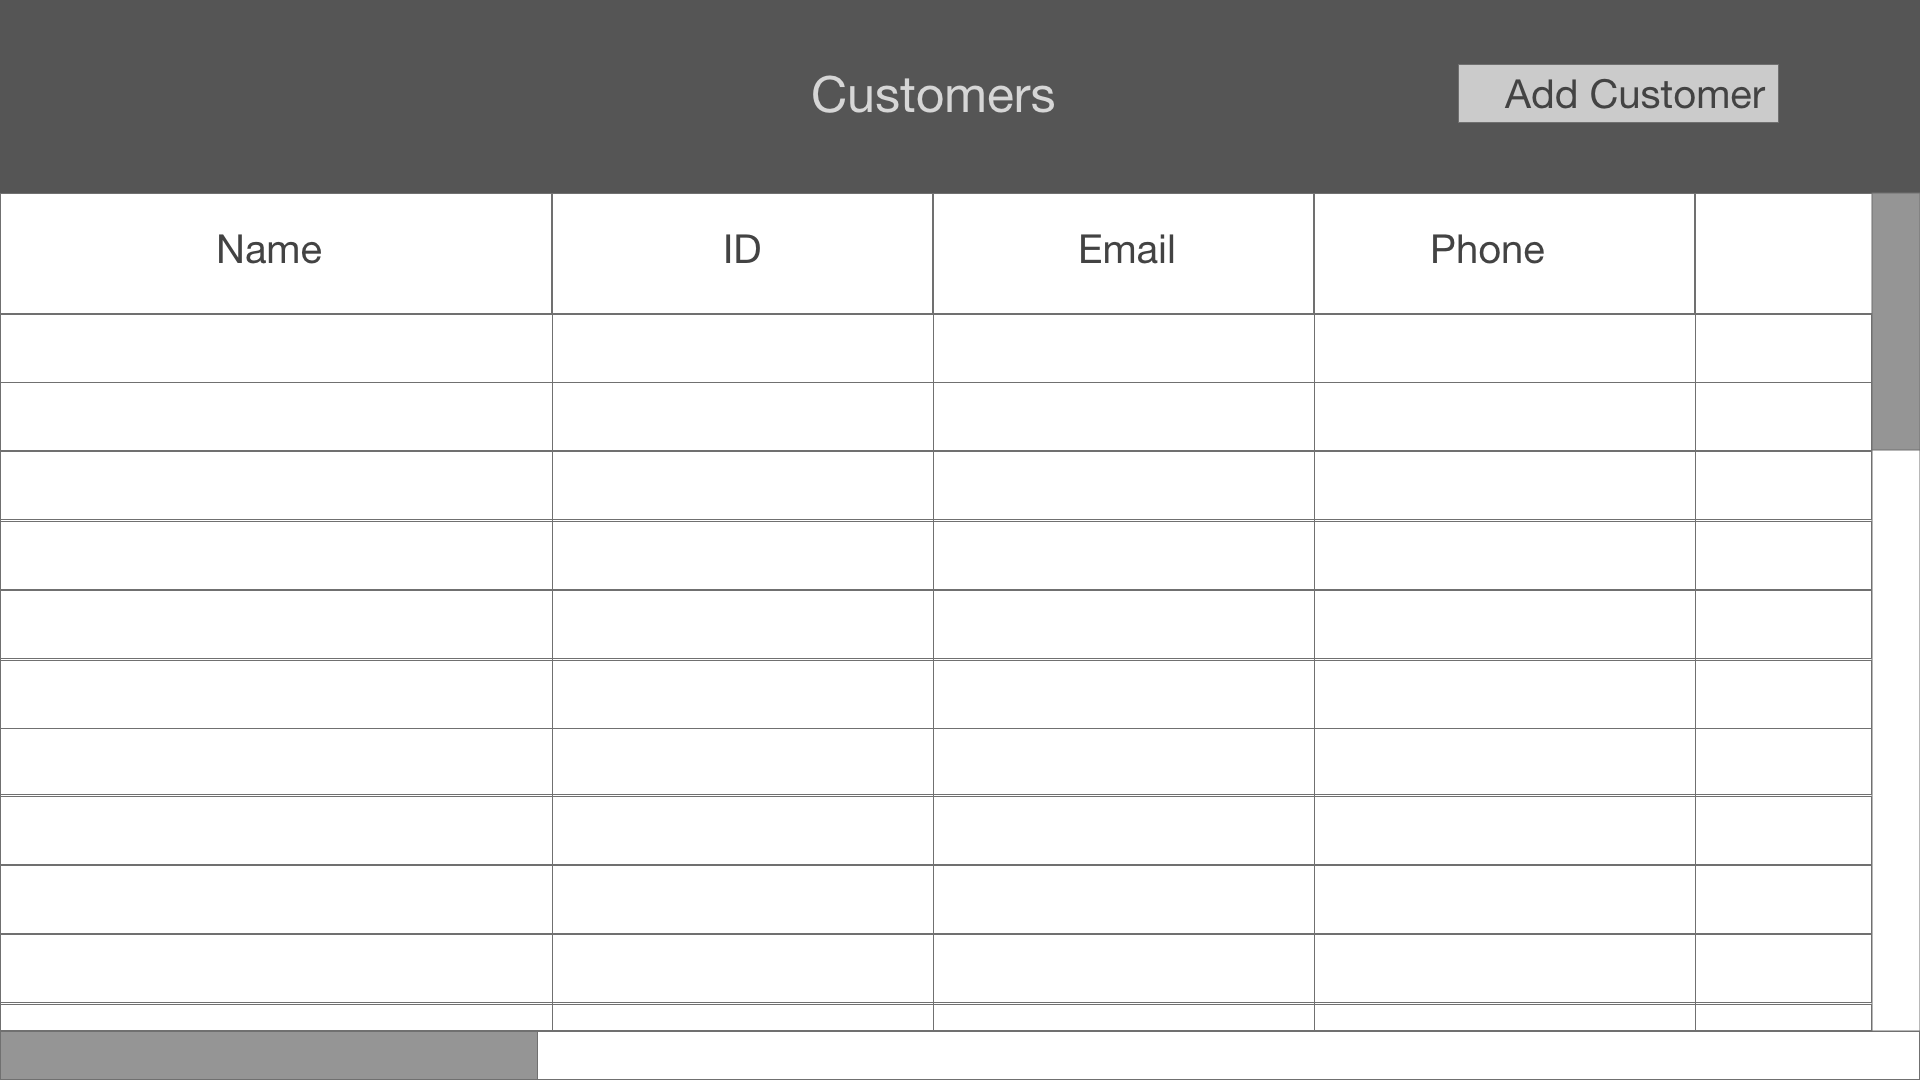
\includegraphics[scale=0.12]{AddCustomer}
	\caption{(2)}
	\end{subfigure}
\end{figure}
\begin{figure}[h]
	\begin{subfigure}{.5\textwidth}
	\centering
	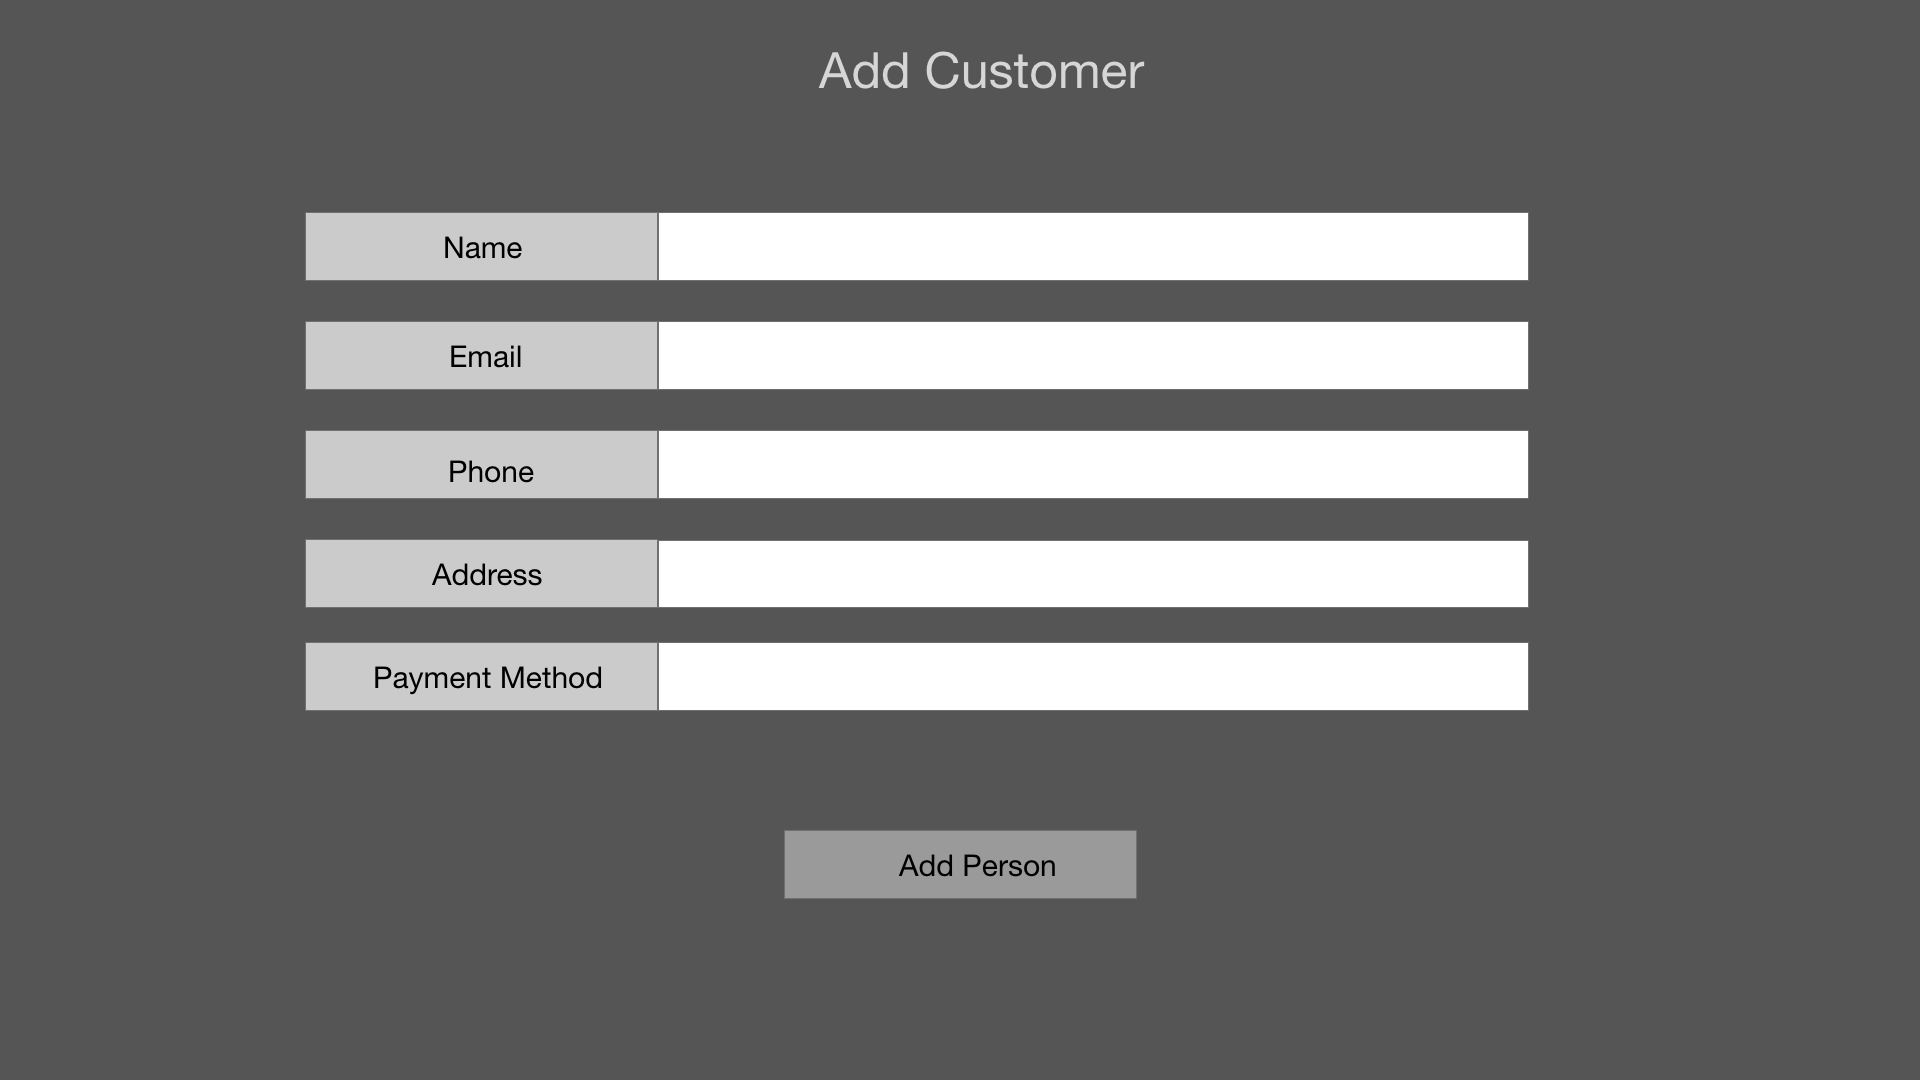
\includegraphics[scale=0.12]{CustInfo}
	\caption{(3)}
	\end{subfigure}%
	\begin{subfigure}{.5\textwidth}
	\centering
	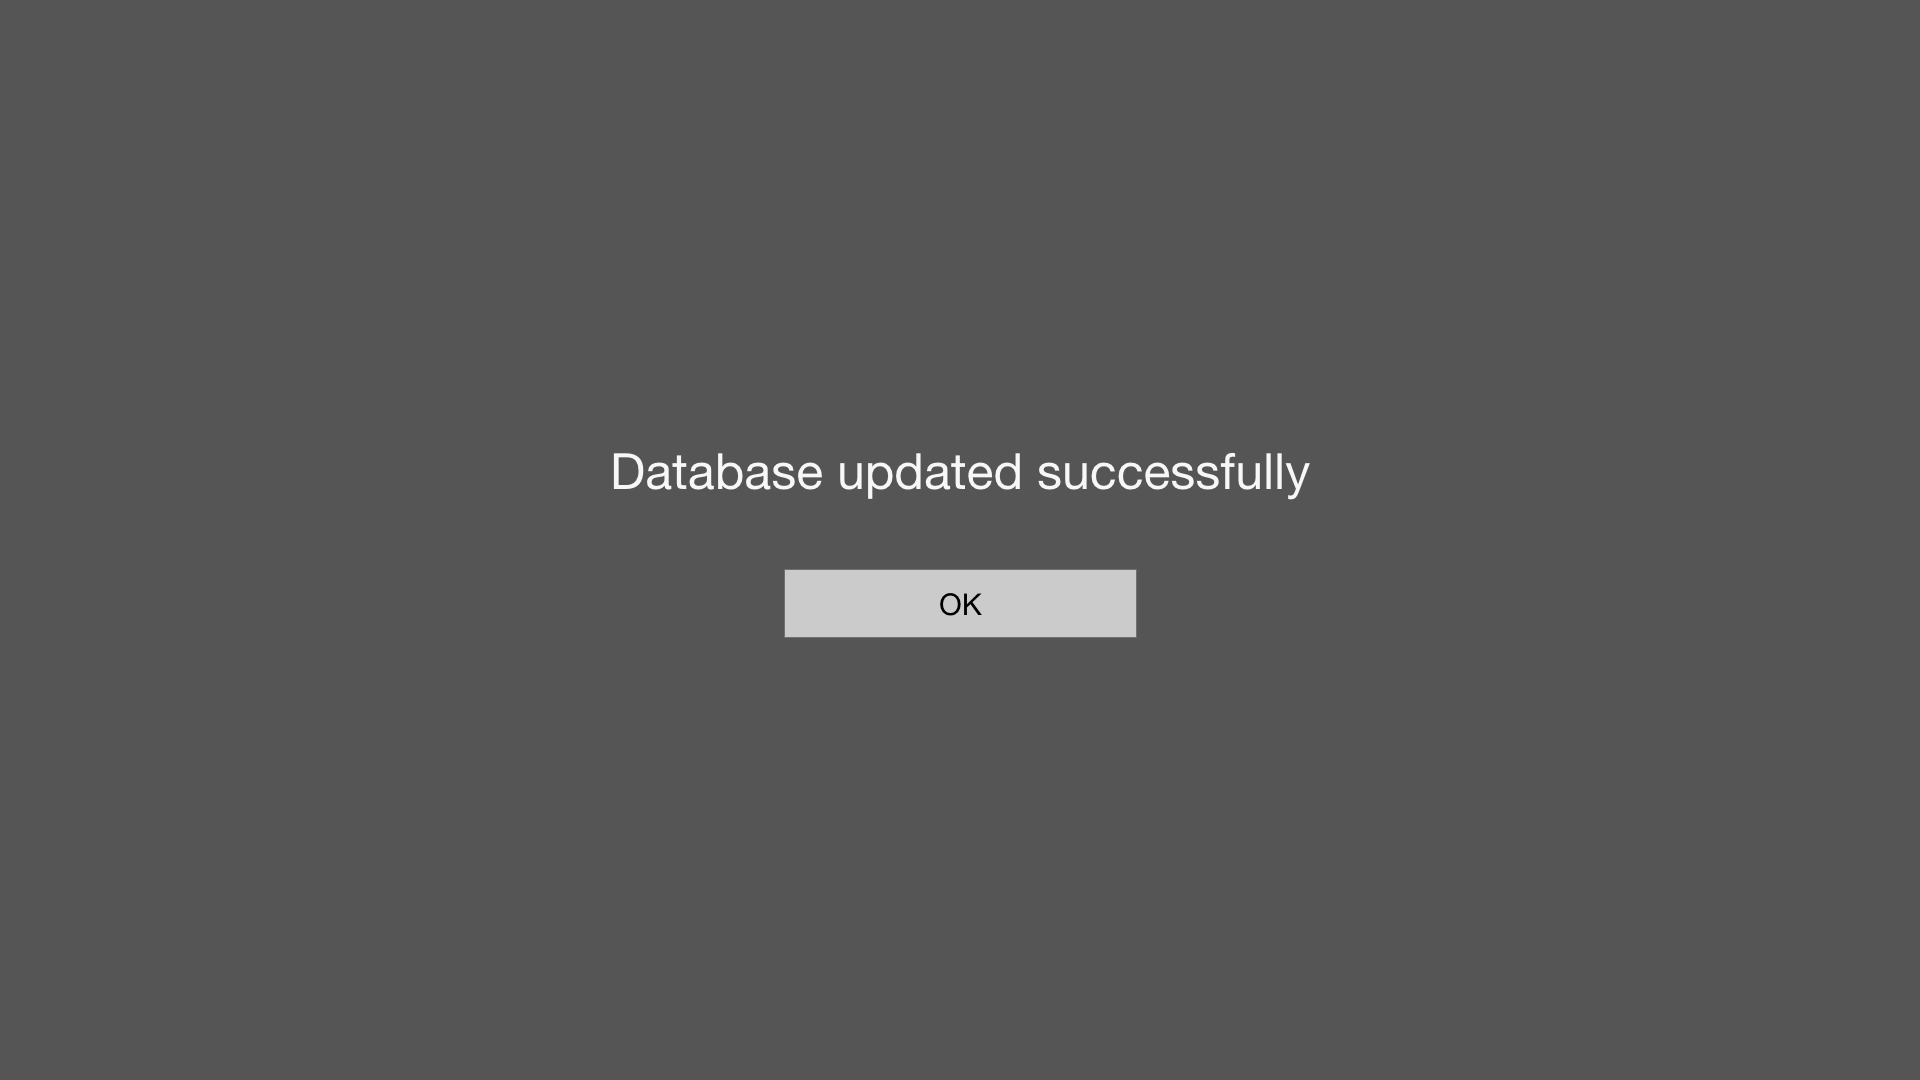
\includegraphics[scale=0.12]{Success}
	\caption{(4)}
	\end{subfigure}
\end{figure}
\newpage
\textbf{Use Case:} update a customer in the system\\
\textbf{Actors:} employees\\
\textbf{Goals:} update a customer entity in the database\\
\textbf{Preconditions:} the specific customer exists in the database\\
\textbf{Postconditions:} the database is updated with desired changes\\
\textbf{steps:}
	\begin{itemize}
		\item[(1)] the user clicks a button to display the customer database
		\item[(2)] the system displays the database
		\item the user (double) clicks on the desired field to edit
		\item the system responds by making the field editable
		\item the user enters desired changes and presses enter
		\item the system updates the underlying database as well as the GUI
	\end{itemize}
the (1) and (2) views here are the same (1) and (2) views on the previous page

\textbf{SQL code} to create table, insert, update, and delete
\begin{lstlisting}
CREATE TABLE IF NOT EXISTS Customer (
	CustomerID integer PRIMARY KEY,
	Name text,
	Email text,
	Phone text,
	Address text,
	PaymentInfo text);
-- Register a new customer named Alice
INSERT INTO Customer (CustomerID, Name, Email, Phone, Address, PaymentInfo)
	VALUES (1, 'Alice', 'a@gmail.com', '555-5555', '1 Main St', 'credit');
-- Alice wishes to change her identity
UPDATE Customer SET 
	CustomerID = 1,
	Name = 'Alice',
	Email = 'a@outlook.com',
	Phone = '666-6666'
	Address = '1 College St',
	PaymentInfo = 'cash',
WHERE CustomerID = 1;
-- Alice wishes to discontinue our services
DELETE FROM Customer WHERE CustomerID = 1;
\end{lstlisting}
\newpage
\section{User Story: Add Transaction}
	\textbf{Use Case:} record a transaction\\
	\textbf{Actors:} employees\\
	\textbf{Goals:} update database to include transaction\\
	\textbf{steps:}
	\begin{itemize}
		\item[(1)] the user clicks a button to record a transaction
		\item[(2)] the system displays a screen with text fields for transaction
		\item the user enters in the information and clicks ok
		\item[(3)] the system displays the receipt with names and prices for confirmation
		\item the user reviews the information and clicks ok
		\item[(4)] the system saves the purchase to the database and displays a success message
	\end{itemize}
\begin{figure}[h]
	\begin{subfigure}{.5\textwidth}
	\centering
	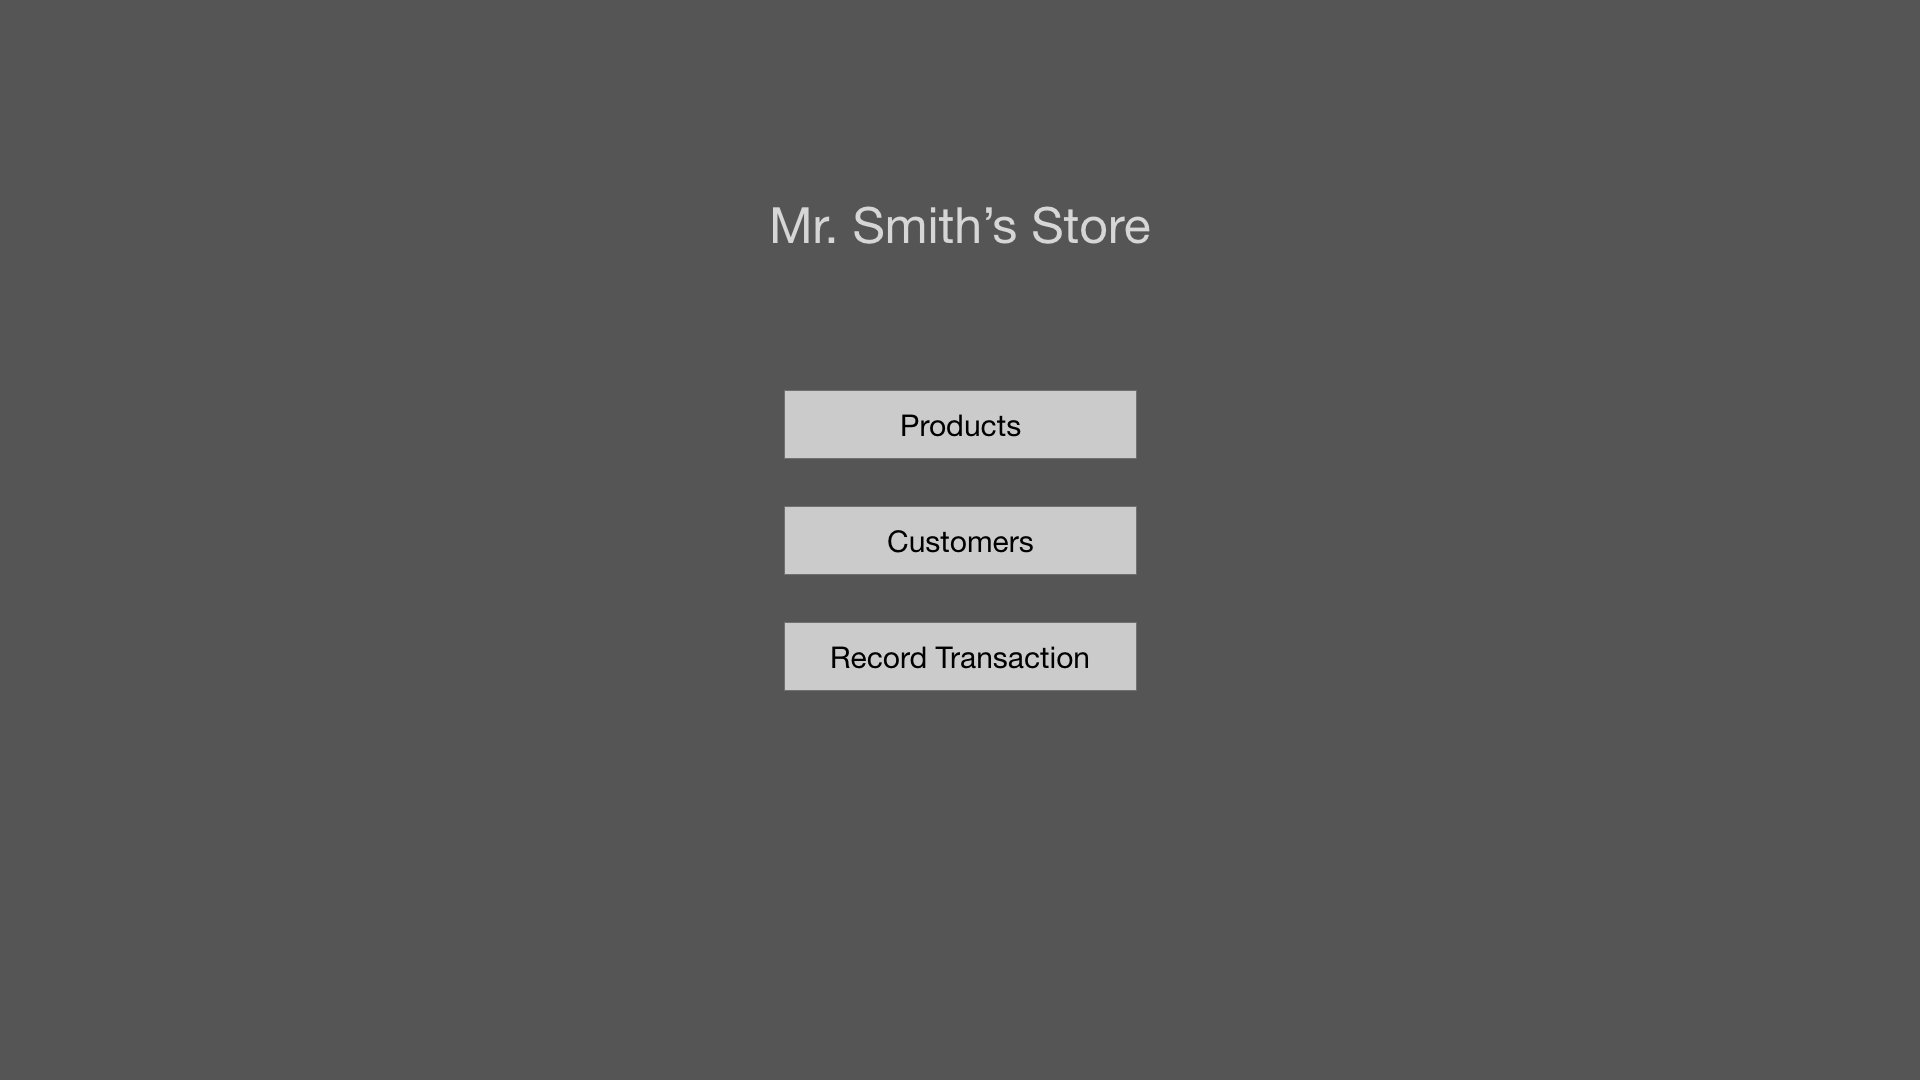
\includegraphics[scale=0.12]{MainMenu}
	\caption{(1)}
	\end{subfigure}%
	\begin{subfigure}{.5\textwidth}
	\centering
	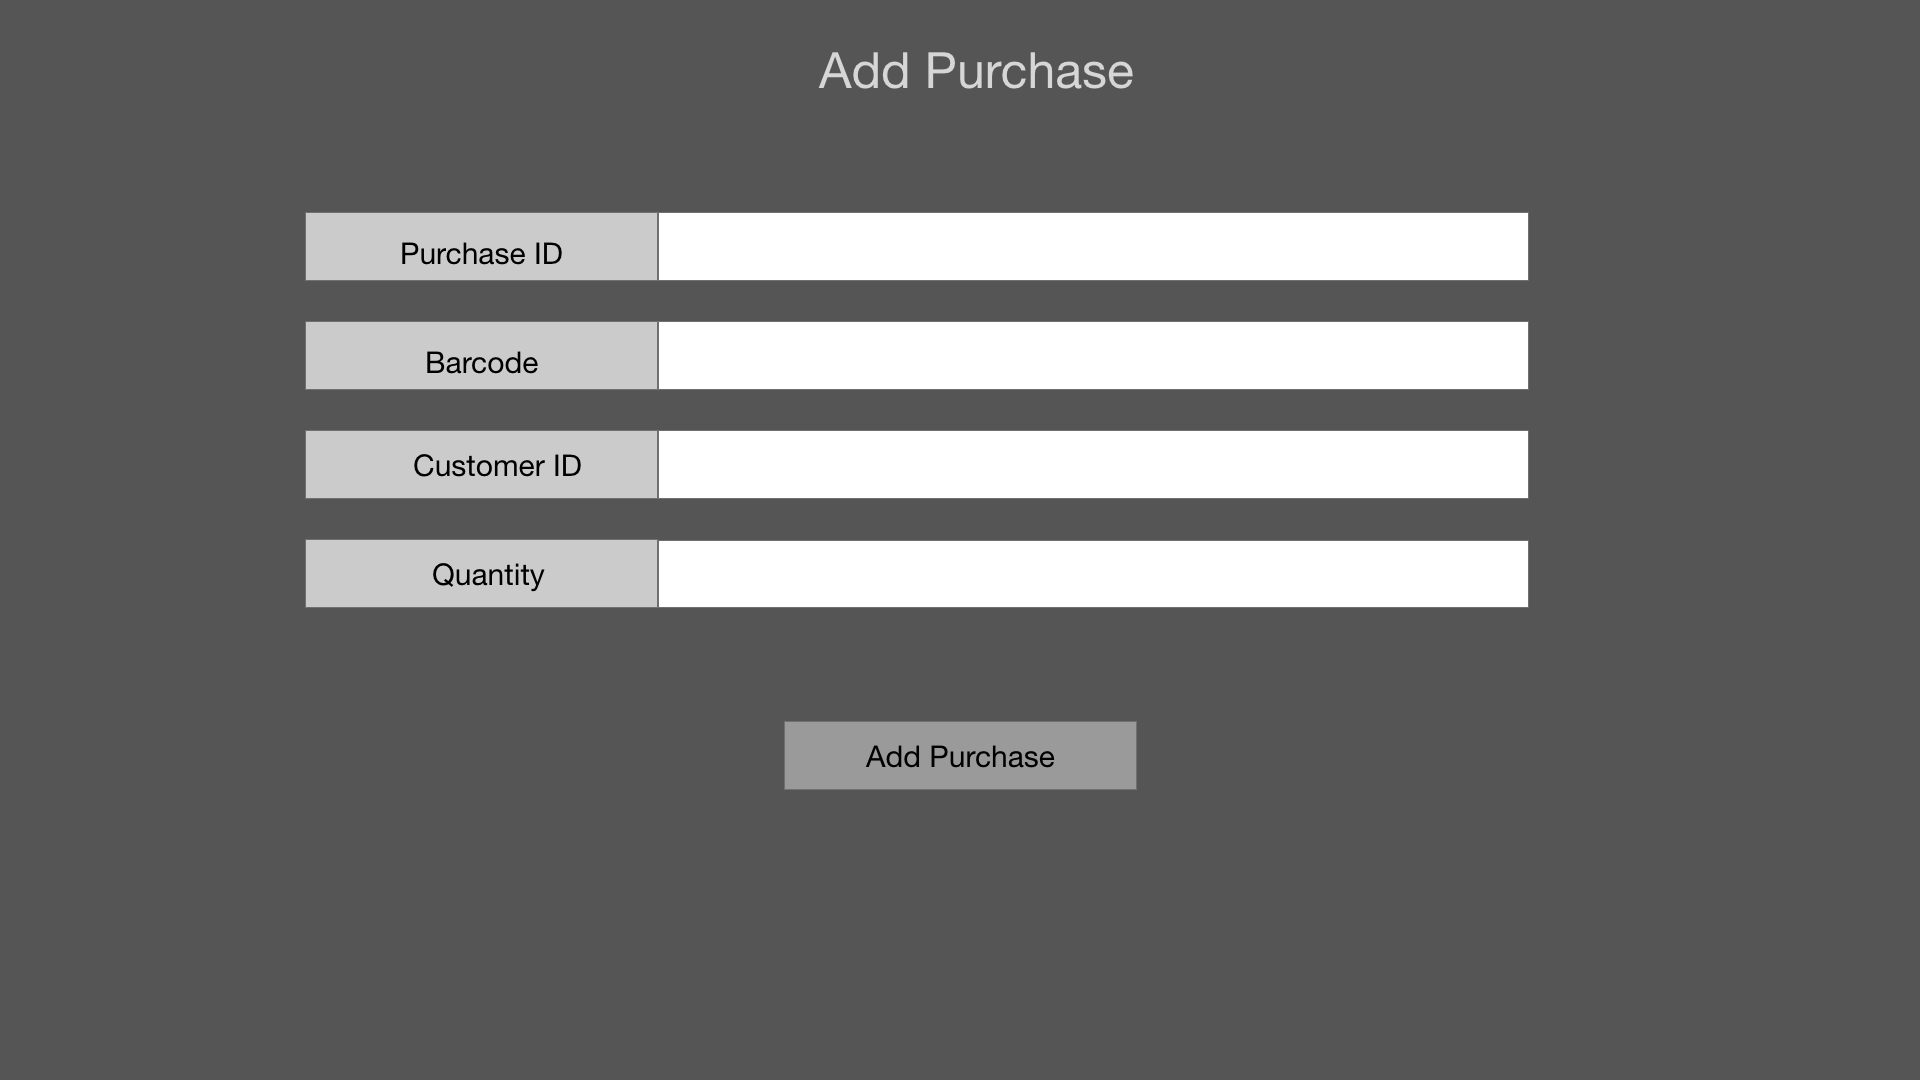
\includegraphics[scale=0.12]{AddPurchase}
	\caption{(2)}
	\end{subfigure}
\end{figure}
\begin{figure}[h]
	\begin{subfigure}{.5\textwidth}
	\centering
	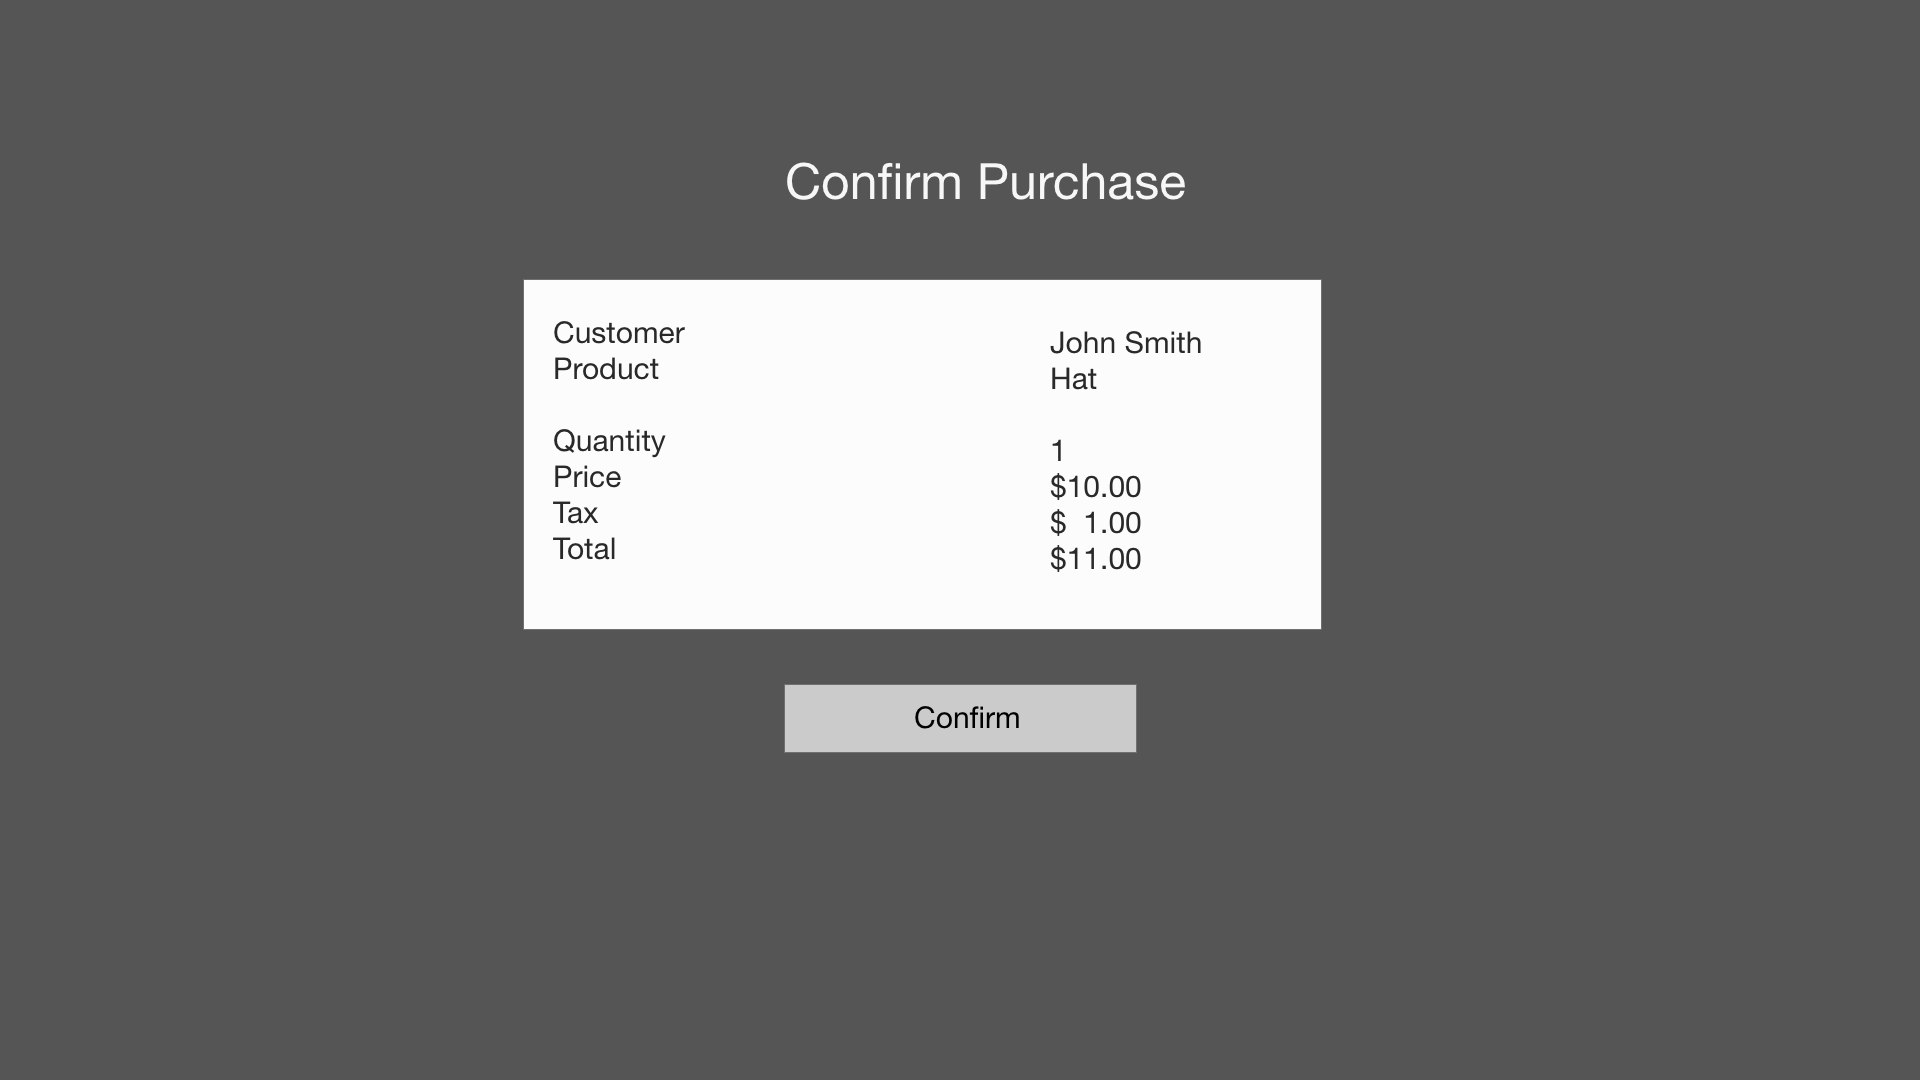
\includegraphics[scale=0.12]{PurchaseConfirm}
	\caption{(3)}
	\end{subfigure}%
	\begin{subfigure}{.5\textwidth}
	\centering
	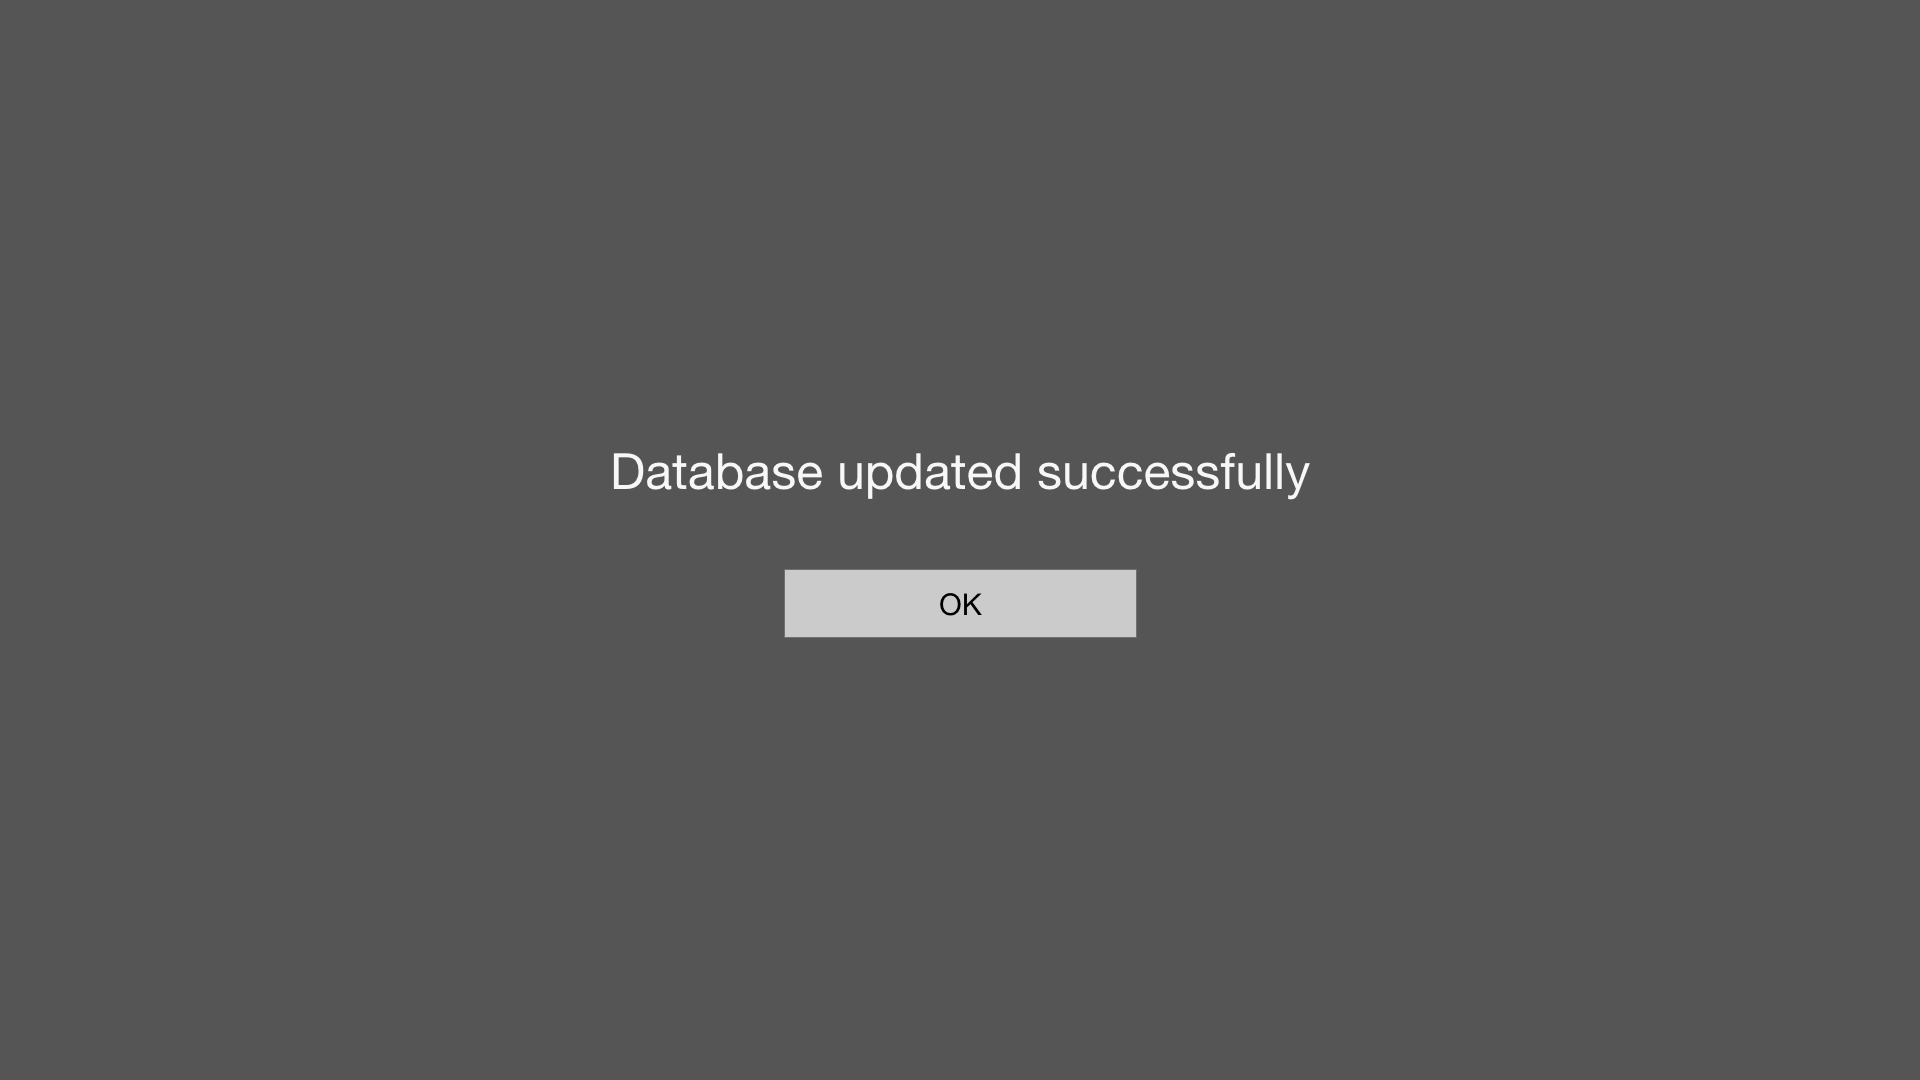
\includegraphics[scale=0.12]{Success}
	\caption{(4)}
	\end{subfigure}
\end{figure}
	\textbf{Use Case:} refund (delete) a transaction\\
	\textbf{Actors:} employees\\
	\textbf{Goals:} delete purchase from database\\
	\textbf{steps:}
	\begin{itemize}
		\item[(1)] the user clicks a button to view transaction database
		\item[(2)] the system displays the purchase database
		\item the user right clicks (or something) on a purchase to delete it
		\item[(3)] the system displays the purchase receipt with a button to delete
		\item the user clicks the delete button
		\item[(2)] the system removes the purchase from the database and updates the view
	\end{itemize}
	Same views as above except the (1) view (main menu) includes a "view transaction" button.
\newpage
\textbf{SQL code} to create table, insert, update, and delete
\begin{lstlisting}
CREATE TABLE IF NOT EXISTS Purchase (
	PurchaseID integer PRIMARY KEY,
	Date text,
	Barcode integer, 
	CustomerID integer,
	Quantity real,
	Price real,
	FOREIGN KEY(Barcode) REFERENCES Product(Barcode),
	FOREIGN KEY(CustomerID) REFERENCES Customer(CustomerID)
	);

-- Price calculated by application based on quantity and product 
-- Date calculated based on current date
INSERT INTO Purchase (PurchaseID, Date, Barcode, CustomerID, Quantity, Price) 
	VALUES (1, '10/16/2019', 1, 1, 5, 999.99);

UPDATE Purchase SET
	PurchaseID = 1,
	Date = '10/16/2019',
	Barcode = 1,
	CustomerID = 1,
	Quantity = 10,
	Price = 1999.98,
WHERE PurchaseID = 1;

-- Issue a refund~\footnote{Disclaimer: the system does not actually issue refunds, the actual transfer of payment must be carried out by the employee operating the system}~
DELETE FROM Purchase WHERE PurchaseID = 1;
\end{lstlisting}
\end{document}